\documentclass[journal,12pt,twocolumn]{IEEEtran}

\usepackage{setspace}
\usepackage{gensymb}

\singlespacing


\usepackage[cmex10]{amsmath}

\usepackage{amsthm}

\usepackage{mathrsfs}
\usepackage{txfonts}
\usepackage{stfloats}
\usepackage{bm}
\usepackage{cite}
\usepackage{cases}
\usepackage{subfig}

\usepackage{longtable}
\usepackage{multirow}

\usepackage{enumitem}
\usepackage{mathtools}
\usepackage{steinmetz}
\usepackage{tikz}
\usepackage{circuitikz}
\usepackage{verbatim}
\usepackage{tfrupee}
\usepackage[breaklinks=true]{hyperref}
\usepackage{graphicx}
\usepackage{tkz-euclide}

\usetikzlibrary{calc,math}
\usepackage{listings}
    \usepackage{color}                                            %%
    \usepackage{array}                                            %%
    \usepackage{longtable}                                        %%
    \usepackage{calc}                                             %%
    \usepackage{multirow}                                         %%
    \usepackage{hhline}                                           %%
    \usepackage{ifthen}                                           %%
    \usepackage{lscape}     
\usepackage{multicol}
\usepackage{chngcntr}

\DeclareMathOperator*{\Res}{Res}

\renewcommand\thesection{\arabic{section}}
\renewcommand\thesubsection{\thesection.\arabic{subsection}}
\renewcommand\thesubsubsection{\thesubsection.\arabic{subsubsection}}

\renewcommand\thesectiondis{\arabic{section}}
\renewcommand\thesubsectiondis{\thesectiondis.\arabic{subsection}}
\renewcommand\thesubsubsectiondis{\thesubsectiondis.\arabic{subsubsection}}


\hyphenation{op-tical net-works semi-conduc-tor}
\def\inputGnumericTable{}                                 %%

\lstset{
%language=C,
frame=single, 
breaklines=true,
columns=fullflexible
}
\begin{document}


\newtheorem{theorem}{Theorem}[section]
\newtheorem{problem}{Problem}
\newtheorem{proposition}{Proposition}[section]
\newtheorem{lemma}{Lemma}[section]
\newtheorem{corollary}[theorem]{Corollary}
\newtheorem{example}{Example}[section]
\newtheorem{definition}[problem]{Definition}

\newcommand{\BEQA}{\begin{eqnarray}}
\newcommand{\EEQA}{\end{eqnarray}}
\newcommand{\define}{\stackrel{\triangle}{=}}
\bibliographystyle{IEEEtran}

\providecommand{\mbf}{\mathbf}
\providecommand{\pr}[1]{\ensuremath{\Pr\left(#1\right)}}
\providecommand{\qfunc}[1]{\ensuremath{Q\left(#1\right)}}
\providecommand{\sbrak}[1]{\ensuremath{{}\left[#1\right]}}
\providecommand{\lsbrak}[1]{\ensuremath{{}\left[#1\right.}}
\providecommand{\rsbrak}[1]{\ensuremath{{}\left.#1\right]}}
\providecommand{\brak}[1]{\ensuremath{\left(#1\right)}}
\providecommand{\lbrak}[1]{\ensuremath{\left(#1\right.}}
\providecommand{\rbrak}[1]{\ensuremath{\left.#1\right)}}
\providecommand{\cbrak}[1]{\ensuremath{\left\{#1\right\}}}
\providecommand{\lcbrak}[1]{\ensuremath{\left\{#1\right.}}
\providecommand{\rcbrak}[1]{\ensuremath{\left.#1\right\}}}
\theoremstyle{remark}
\newtheorem{rem}{Remark}
\newcommand{\sgn}{\mathop{\mathrm{sgn}}}
\providecommand{\abs}[1]{\left\vert#1\right\vert}
\providecommand{\res}[1]{\Res\displaylimits_{#1}} 
\providecommand{\norm}[1]{\left\lVert#1\right\rVert}
%\providecommand{\norm}[1]{\lVert#1\rVert}
\providecommand{\mtx}[1]{\mathbf{#1}}
\providecommand{\mean}[1]{E\left[ #1 \right]}
\providecommand{\fourier}{\overset{\mathcal{F}}{ \rightleftharpoons}}
%\providecommand{\hilbert}{\overset{\mathcal{H}}{ \rightleftharpoons}}
\providecommand{\system}{\overset{\mathcal{H}}{ \longleftrightarrow}}
	%\newcommand{\solution}[2]{\textbf{Solution:}{#1}}
\newcommand{\solution}{\noindent \textbf{Solution: }}
\newcommand{\cosec}{\,\text{cosec}\,}
\providecommand{\dec}[2]{\ensuremath{\overset{#1}{\underset{#2}{\gtrless}}}}
\newcommand{\myvec}[1]{\ensuremath{\begin{pmatrix}#1\end{pmatrix}}}
\newcommand{\mydet}[1]{\ensuremath{\begin{vmatrix}#1\end{vmatrix}}}
\numberwithin{equation}{subsection}

\makeatletter
\@addtoreset{figure}{problem}
\makeatother
\let\StandardTheFigure\thefigure
\let\vec\mathbf

\renewcommand{\thefigure}{\theproblem}

\def\putbox#1#2#3{\makebox[0in][l]{\makebox[#1][l]{}\raisebox{\baselineskip}[0in][0in]{\raisebox{#2}[0in][0in]{#3}}}}
     \def\rightbox#1{\makebox[0in][r]{#1}}
     \def\centbox#1{\makebox[0in]{#1}}
     \def\topbox#1{\raisebox{-\baselineskip}[0in][0in]{#1}}
     \def\midbox#1{\raisebox{-0.5\baselineskip}[0in][0in]{#1}}
\vspace{3cm}
\title{Assignment 5}
\author{Sachinkumar Dubey - EE20MTECH11009}

\maketitle
\newpage
\bigskip
\renewcommand{\thefigure}{\theenumi}
\renewcommand{\thetable}{\theenumi}
Download all python codes from 
\begin{lstlisting}
https://github.com/sachinomdubey/Matrix-theory/Assignment5/codes
\end{lstlisting}
%
and latex-tikz codes from 
%
\begin{lstlisting}
https://github.com/sachinomdubey/Matrix-theory/Assignment5
\end{lstlisting}
\subsection{Problem}
(Geolin 1.9) $AB$ is a line-segment. $P$ and $Q$ are points on opposite sides of $AB$ such that each of them is equidistant from the points $A$ and $B$. Show that the line $PQ $ is the perpendicular bisector of $AB$.
\\
\begin{figure}[h!]
\centering
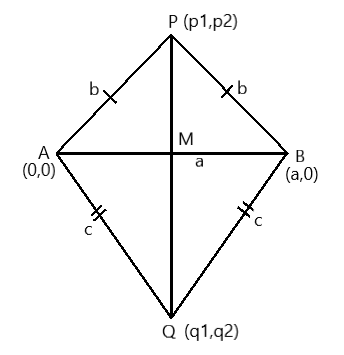
\includegraphics[width=7cm, height=7cm]{Figure_51}
\caption{}
\label{Fig4}
\end{figure}
\\
\subsection{Explanation}
In order to prove that line $PQ $ is the perpendicular bisector of $AB$, two conditions need to be met:
\begin{enumerate}
    \item $AM$=$BM$
    \item $PM \perp AB $
\end{enumerate}
These conditions can be proved using cosine law in vector form and some vector theory. The solution is as follow:
\subsection{Solution}
It is given that the points $\vec{P}$ and $\vec{Q}$  are equidistant from the points $\vec{A}$ and $\vec{B}$. Thus we can write:
\begin{align}
    \norm{\vec{PA}}=\norm{\vec{PB}} \label{eq2.2}\\
    \norm{\vec{QA}}=\norm{\vec{QB}} \label{eq2.3}
\end{align}
Using the law of cosine, we can write:
\begin{align}
    \norm{\vec{AQ}}^2= \norm{\vec{PA}}^2+ \norm{\vec{PQ}}^2-2 \norm{\vec{PA}} \norm{\vec{PQ}}cos \Theta \label{eq3.3}\\
    \norm{\vec{BQ}}^2= \norm{\vec{PB}}^2+ \norm{\vec{PQ}}^2-2 \norm{\vec{PB}} \norm{\vec{PQ}}cos \phi \label{eq3.4}
\end{align}
From equations \ref{eq2.2} \ref{eq2.3} \ref{eq3.3} and \ref{eq3.4}, we can write:
\begin{align}
    cos \Theta = cos \phi \\
    \therefore \implies \Theta = \phi \label{eq3.6}
\end{align}
Again using the law of cosine, we can write:
\begin{align}
    \norm{\vec{AM}}^2= \norm{\vec{PA}}^2+ \norm{\vec{PM}}^2-2 \norm{\vec{PA}} \norm{\vec{PM}}cos \Theta \label{eq3.7}\\
    \norm{\vec{BM}}^2= \norm{\vec{PB}}^2+ \norm{\vec{PM}}^2-2 \norm{\vec{PB}} \norm{\vec{PM}}cos \phi \label{eq3.8}
\end{align}
From equations \ref{eq2.2} and \ref{eq3.6}, we can write:
\begin{align}
  \norm{\vec{BM}}^2= \norm{\vec{PA}}^2+ \norm{\vec{PM}}^2-2 \norm{\vec{PA}} \norm{\vec{PM}}cos \Theta  \label{eq3.9}
\end{align}
From equations \ref{eq3.7} and \ref{eq3.9}, we can write:
\begin{align}
    \norm{\vec{AM}}^2=\norm{\vec{BM}}^2 \\
    \therefore \norm{\vec{AM}}=\norm{\vec{BM}}
\end{align}
Thus, Segment $PQ$ bisects segment $AB$. \\
From the figure, the vector $\vec{AB}$ can be written as:
\begin{align}
\vec{AB}=\vec{AP}+\vec{PB} \label{eq3.12}
\end{align}
Also, the vector $\vec{PM}$ can be written as:
\begin{align}
\vec{PM}=\vec{PA}+\vec{AM}
\end{align}
The point $M$ is the midpoint of the segment $AB$, therefore the vector $\vec{AM}$ is :
\begin{align}
    \vec{AM}=\frac{1}{2}\Vec{AB}\\
    \therefore \vec{PM}=\vec{PA}+\frac{1}{2}\Vec{AB}
\end{align}
From equation \ref{eq3.12}:
\begin{align}
    \vec{PM}=\vec{PA}+\frac{1}{2}(\vec{AP}+\vec{PB})\\
     \vec{PM}=\vec{PA}+\frac{1}{2}\vec{AP}+\frac{1}{2}\vec{PB}\\
     \vec{PM}=\vec{PA}-\frac{1}{2}\vec{PA}+\frac{1}{2}\vec{PB}\\
     \vec{PM}=\frac{1}{2}(\vec{PA}+\vec{PB}) \label{eq3.19}
\end{align}
For $PM \perp AB $, The dot product of vectors $\Vec{AB}$ and $\Vec{PM}$ should be zero. Using equations \ref{eq3.12} and \ref{eq3.19}:
\begin{align}
    \vec{AC}^T\vec{PM}=(\vec{AP}+\vec{PB})^T\frac{1}{2}(\vec{PA}+\vec{PB})\\
     \vec{AC}^T\vec{PM}=\frac{1}{2}(\vec{AP}^T+\vec{PB}^T)(\vec{PA}+\vec{PB})\\
     \vec{AC}^T\vec{PM}=\frac{1}{2}(-\vec{PA}^T+\vec{PB}^T)(\vec{PA}+\vec{PB})\\
     \vec{AC}^T\vec{PM}=\frac{1}{2}(\vec{PB}^T\vec{PB}-\vec{PA}^T\vec{PA})
\end{align}
\begin{align}
     \vec{AC}^T\vec{PM}=\frac{1}{2}(\norm{\vec{PB}}^2-\norm{\vec{PA}}^2)\\
     \vec{AC}^T\vec{PM}=0
\end{align}
Thus, Segment $PQ$ is perpendicular bisector of segment $AB$.
\end{document}